\documentclass{standalone}
\usepackage{tikz}

\begin{document}

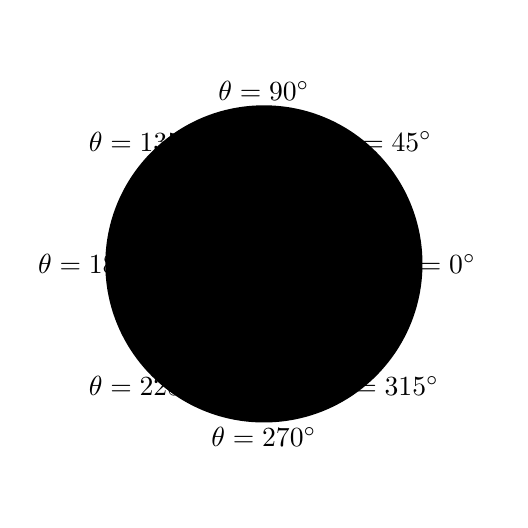
\begin{tikzpicture}[scale=1]
    % Set up the white background
    \fill[white] (-3,-3) rectangle (3,3);

    % Draw the circle with radius 2 and fill it with dark color (black)
    \draw[thick, fill=black] (0,0) circle (2cm);
    
    % Label the circle with values of t (polar coordinates)
    \foreach \angle in {0,45,90,135,180,225,270,315} {
        \node at (\angle:2.2) {\(\theta = \angle^\circ\)};
    }
\end{tikzpicture}

\end{document}